\documentclass[12pt,a4paper,titlepage]{article}
\title{Confronto fra algoritmo LMS e Fast Deconvolution per la cancellazione del crosstalk} 
\author{Matteo Orlandini}
\date{\today}

\usepackage[english, italian]{babel} %the last declared language is the one used in the document
\usepackage[utf8]{inputenc}
\usepackage[T1]{fontenc}
\usepackage{booktabs} %toprule, midrule, bottomrule
\usepackage{subfig}
\usepackage{graphicx}
\usepackage{listings}
\usepackage{siunitx}
\usepackage{amsmath}
\usepackage{mcode} % matlab code
%inizio impostazioni bibliografia
\usepackage[autostyle,italian=guillemets]{csquotes} 
%autostyle adatta lo stile delle citazioni alla lingua corrente del documento;
%italian=guillemets racchiude automaticamente tra virgolette caporali
%i campi che prevedono le virgolette;
\usepackage[backend=biber, style=numeric, citestyle=numeric,maxcitenames=99,maxbibnames = 99]{biblatex}
%backend=biber dice a biblatex che s’intende usare Biber come motore bibliografico
%style:numeric Anno di pubblicazione: in fondo al riferimento.
%citestyle=numeric Riferimento: numerico ([1], [2], eccetera).
%fine impostazioni bibliografia

\usepackage{float}
\usepackage{hyperref}
\hypersetup{
	bookmarks=true,         % show bookmarks bar?
	unicode=false,          % non-Latin characters in Acrobat’s bookmarks
	pdftoolbar=true,        % show Acrobat’s toolbar?
	pdfmenubar=true,        % show Acrobat’s menu?
	pdffitwindow=false,     % window fit to page when opened
	pdfstartview={FitH},    % fits the width of the page to the window
	%pdftitle={Relazione di Reti di Sensori Wireless per IOT},    % title
	pdfauthor={Matteo Orlandini},     % author
	pdfsubject= {Confronto fra algoritmo LMS e Fast Deconvolution per la cancellazione del crosstalk},   % subject of the document
	pdfcreator={Matteo Orlandini},   % creator of the document
	%pdfproducer={Producer}, % producer of the document
	pdfpagemode={UseOutlines},
	%bookmarksopen,
	pdfstartview={FitH},
	colorlinks=false,       % false: boxed links; true: colored links
	linkcolor={red},
	citecolor={green},
	urlcolor={cyan}
} 

\renewcommand{\lstlistingname}{Codice}

\addbibresource{Bibliografia.bib}

\newcommand{\CoverName}{Cover}

\begin{document}

\begin{titlepage}
	
	\centering
	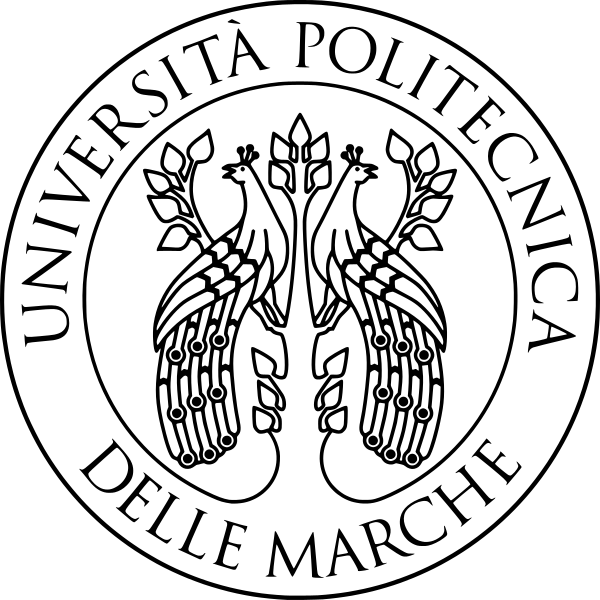
\includegraphics[width=.2\textwidth]{Immagini/univpmlogo}\par\vspace{1cm}
	{\scshape\LARGE Università Politecnica delle Marche\par}
	\vspace{1cm}
	{\scshape\Large Multirate Digital Signal Processing And Adaptive Filter Banks \par}
	\vspace{1.5cm}
	{\huge\bfseries Confronto fra algoritmo LMS e Fast Deconvolution per la cancellazione del crosstalk \par}
	\vspace{2cm}
	{\Large\itshape Matteo Orlandini e Jacopo Pagliuca\par}
	\vfill
	Prof.ssa Stefania \textsc{Cecchi}\\
	Dott.ssa Valeria \textsc{Bruschi}
	
	\vfill
	
	% Bottom of the page
	{\large \today\par}
\end{titlepage}

\thispagestyle{empty}
\tableofcontents

\newpage
\setcounter{page}{1}
\section{Introduzione}
\label{sec:Introduzione}
\clearpage

\section{Dataset}
\label{sec:Dataset}
Il dataset usato è composto ad un ampio set di \href{http://sound.media.mit.edu/resources/KEMAR/full.zip}{misurazioni della funzione di trasferimento relativa alla testa} (HRTF) di un microfono dummy-head KEMAR. Le misurazioni consistono nelle risposte impulsive dell'orecchio sinistro e destro di un altoparlante Realistic Optimus Pro 7 montato a 1,4 metri dal KEMAR. Sono state utilizzate sequenze binarie pseudo-casuali per ottenere le risposte impulsive a una frequenza di campionamento di \SI{44.1}{\kilo \hertz}. \cite{Gardner:HRTF}

Le misurazioni sono state effettuate nella camera anecoica del MIT. Il KEMAR è stato montato in posizione verticale su un giradischi motorizzato che può essere ruotato con precisione sotto il controllo del computer. L'altoparlante è stato montato su un supporto a braccio che ha consentito il posizionamento accurato dell'altoparlante a qualsiasi elevazione rispetto al KEMAR. Pertanto, le misurazioni sono state effettuate un'elevazione alla volta, impostando l'altoparlante all'altezza corretta e quindi ruotando il KEMAR su ciascun azimut.

I dati HRTF vengono archiviati nelle directory per elevazione. Ogni nome di directory ha il formato "elevEE", dove EE è l'angolo di elevazione. All'interno di ogni directory, il nome di ogni file ha il formato "XEEeAAAa.wav" dove X può essere "L" o "R" rispettivamente per la risposta dell'orecchio sinistro e destro, "EE" è l'angolo di elevazione della sorgente in gradi, da -40° a 90°, e AAA è l'azimut della sorgente in gradi, da 0° a 355°. Gli angoli di elevazione e azimut indicano la posizione della sorgente rispetto al KEMAR, in modo che, ad esempio, in corrispondenza dell'elevazione 0 e azimut 0 sia di fronte al KEMAR , l'elevazione 90 è direttamente sopra il KEMAR, elevazione 0 e azimut 90 è a destra del KEMAR. Ad esempio, il file "R-20e270a.wav" è la risposta dell'orecchio destro, con la sorgente 20 gradi sotto il piano orizzontale e 90 gradi a sinistra della testa.
\clearpage
\section{Descrizione teorica degli algoritmi}
\label{sec:descrizione_teorica}
\subsection{LMS}
\label{subsec:LMS_teoria}

\subsection{Fast Deconvolution}
\label{subsec:FD_teoria}
La deconvoluzione~\cite{kirkeby:deconvolution_regularization}~\cite{kirkeby:deconvolution_analysis}~\cite{kirkeby:deconvolution_design}, nella sua forma più elementare, può essere descritta come il compito di calcolare l'input di un sistema a tempo discreto conoscendo il suo output. Di solito si presume che il sistema sia lineare e che la relazione input output sia nota con precisione. In acustica e audio, la deconvoluzione a singolo canale è particolarmente utile poiché può compensare la risposta di trasduttori imperfetti come cuffie, altoparlanti e amplificatori. La deconvoluzione multicanale è necessaria nella progettazione di sistemi di cancellazione della diafonia e sistemi di imaging di sorgenti virtuali.%~\cite{kirkeby:deconvolution_analysis}

Nel progetto siamo interessati alle tecniche di deconvoluzione allo scopo di progettare filtri digitali per la riproduzione del suono su due canali. Più specificamente, dato un set di altoparlanti S, l'obiettivo è riprodurre un campo sonoro desiderato nei punti R dello spazio nel modo più accurato possibile. Questo principio è applicato dai cosiddetti sistemi di cancellazione della diafonia che vengono utilizzati per riprodurre registrazioni binaurali su due altoparlanti. In questo caso, viene utilizzata una matrice $2 \times 2$ di filtri digitali per compensare sia la risposta ambientale che la risposta degli altoparlanti, e anche per annullare la diafonia dall'altoparlante sinistro all'orecchio destro e viceversa. Un problema correlato è quello di ottenere una perfetta ``dereverberazione'' della risposta di una stanza in una posizione del microfono utilizzando due filtri digitali per calcolare l'ingresso a due altoparlanti. La fast deconvolution un metodo molto veloce per calcolare una matrice di filtri digitali che può essere utilizzata per controllare le uscite di un impianto multicanale. Questo metodo è tipicamente più veloce di diversi ordini di grandezza rispetto ai metodi nel dominio del tempo. Combina i principi dell'inversione dei minimi quadrati nel dominio della frequenza e il metodo di regolarizzazione di ordine zero che viene tradizionalmente utilizzato quando ci si trova di fronte a un problema di inversione mal condizionata.%~\cite{kirkeby:deconvolution_regularization}

La regolarizzazione dipendente dalla frequenza viene utilizzata per prevenire picchi elevati nella risposta in ampiezza dei filtri ottimali. Un ritardo di modellazione viene utilizzato per garantire che la rete di cancellazione del cross-talk funzioni bene non solo in termini di ampiezza, ma anche in termini di fase. L'algoritmo presuppone che sia possibile utilizzare filtri ottimali lunghi, e funziona bene solo quando due parametri di regolarizzazione, un fattore di forma e un fattore di guadagno, sono impostati in modo appropriato. In pratica, i valori dei due parametri di regolarizzazione sono determinati più facilmente da esperimenti per tentativi.%~\cite{kirkeby:deconvolution_design}

Consideriamo una funzione di costo del tipo
\begin{equation}\label{funzione_costo_fd}
J = E + \beta V(f)
\end{equation}
dove $E$ è una misura dell'errore della pressione sonora
\begin{equation}\label{errore_fd}
E = | Y_1 - X_1 |^2  + | Y_2 - X_2 |^2
\end{equation}
e $V$ è una funzione della frequenza che indica il costo computazionale. Il numero $\beta \geq 0$ è un parametro di regolarizzazione che determina quanto peso
assegnare alla funzione $V$. Poiché non sappiamo a priori se la matrice $C$ è non singolare per determinate frequenze, la matrice $H$ di cancellazione del crosstalk può contenere valori molto alti. All'aumentare di $\beta$ da zero a infinito, $J$ cambia gradualmente dalla minimizzazione della sola funzione di errore $E$ alla minimizzazione dello sforzo computazionale $V$.

Siano $S$ i segnali trasferiti agli altoparlanti facendo passare il segnale $X$ attraverso la matrice di cancellazione del crosstalk $H$. Otteniamo
\begin{equation}
V(f) = S_b ^{+} S_b
\end{equation}
con
\begin{equation}
S_b = BS = BHX
\end{equation}
dove $B$ è una matrice $2 \times 2$ e il simbolo $+$ indica l'inversa generalizzata della matrice $S_b$. La soluzione approssimata della funzione $J$ è definita da 
\begin{equation}\label{eq:H_FD}
H(z) = \left[C^T (z^{-1}) C(z) + \beta B^T B)\right]^{-1} C^T(z^{-1})
\end{equation}
dove l'apice $T$ denota la trasposta della matrice. Se la matrice $B$ è uguale alla matrice identità $I$, si ottiene $S_b = S$, dunque l'equazione~\eqref{eq:H_FD} diventa
\begin{equation}\label{eq:H_FD2}
H(z) = \left[C^T (z^{-1}) C(z) + \beta I)\right]^{-1} C^T(z^{-1}) z^{-m}
\end{equation}
dove la componente $z^{-m}$ implementa un ritardo di $m$ campioni.

Le equazioni~\eqref{eq:H_FD} e~\eqref{eq:H_FD2} rappresentano una espressione di $H(z)$ nel dominio continuo della frequenza. Se viene usata una FFT a $N$ punti per campionare la risposta in frequenza $H(z)$, allora il valore di $H[k]$ è dato da
\begin{equation}\label{H_FD_3}
H[k] = \left[C^H[k] C[k] + \beta I)\right]^{-1} C^H[k]
\end{equation}
dove $k$ indica la $k$-esima frequenza corrispondente a $\exp(j2\pi k/N)$ e l'apice $H$ denota l'operatore Hermitiano che fa la trasposta coniugata del suo argomento. Dall'equazione~\eqref{H_FD_3} si può osservare che ponendo $\beta = 0$ si ottiene $H = C^{-1}$. In questo caso, poiché $Y = CHX = C C^{-1} X = IX = X$, si ottiene in uscita il segnale d'ingresso.

Per calcolare la risposta impulsiva del filtro occorre seguire i seguenti passi:
\begin{enumerate}
\item si calcola la matrice $2 \times 2$ $C[k]$ tramite una FFT delle risposte impulsive $c_{ij}[n]$ con $i = 1, 2$ e $j = 1, 2$. Ad esempio, $C_{11}[k]$ contiene l'ampiezza della $k$-esima armonica della FFT di $c_{11}$,
\item si calcola $H[k]$ usando la formula~\eqref{H_FD_3},
\item si calcola $h[n]$ facendo una FFT inversa a $N$ punti,
\item si implementa uno shift ciclico di $m$ campioni per ogni elemento di $h_{ij}[n]$ con $i = 1, 2$ e $j = 1, 2$.
\end{enumerate}

Dato che l'uscita $Y$ è data da
\begin{equation}\label{eq:y_matrix}
Y = CHX = 
\begin{bmatrix}
C_{11} X_1 & C_{12} X_1 & C_{11} X_2 & C_{12} X_2 \\ 
C_{21} X_1 & C_{22} X_1 & C_{21} X_2 & C_{22} X_2 \\ 
\end{bmatrix}
\begin{bmatrix}
H_{11}\\
H_{21}\\
H_{12}\\
H_{22}\\
\end{bmatrix}
\end{equation}
nell'implementazione pratica non si può calcolare tutta l'uscita con la sola operazione matriciale~\eqref{eq:y_matrix}, occorre usare la tecnica dell'overlap and save per filtrare l'ingresso $X$ con i filtri $C$ e $H$. L'overlap and save è utile per eseguire un filtraggio in real time con un filtro a risposta impulsiva finita. Questa tecnica viene usata per fare la convoluzione a blocchi tra un segnale di ingresso $x[n]$ molto lungo e un filtro FIR $h[n]$:
\begin{equation}
y[n] = x[n] * h[n] = \sum_{m=-\infty}^{+\infty} {h[m] \cdot x[n-m]} = \sum_{m=1}^{M} {h[m] \cdot x[n-m]}
\end{equation}
poiché $h[m]$ = 0 per $m \in [1, M]$.

L'overlap and save permette di calcolare dei blocchi di $y[n]$ di lunghezza $L$ e concatenarli insieme per formare il segnale di uscita completo. Si definisce il $k$-esimo blocco d'ingresso come
\begin{equation}
x_k[n] = 
\begin{cases}
x[n+kL], & 1 \leq n \leq L + M - 1\\
0 & \text{altrove}
\end{cases}
\end{equation}
quindi il $k$-esimo blocco di uscita è dato da 
\begin{equation}
y_k[n] = x_k[n] * h[n] = \sum_{m=1}^{M} {h[m] \cdot x_k[n-m]}.
\end{equation}
Si può definire l'uscita per $kL + M \leq n \leq KL + L +M - 1$, o in modo equivalente per $M \leq n - kL \leq L + M - 1$, nel seguente modo:
\begin{equation}
y[n] = \sum_{m=1}^{M} {h[m] \cdot x_k[n-kL-m]} = y_k[n - kL].
\end{equation}
L'implementazione dell'overlap and save con un filtro composto da $(L + M - 1)$ tappi consiste nei seguenti passi:
\begin{enumerate}
\item si divide il segnale di ingresso in blocchi di lunghezza $L$
\item nel caso del primo blocco si aggiungono $M - 1$ zeri all'inizio, altrimenti si aggiungono all'inizio del blocco gli ultimi $M - 1$ campioni del blocco precedente, come mostrato in figura~\ref{fig:ols},
\item si fa la FFT a $L + M - 1$ punti del $k$-esimo blocco di ingresso,
\item si fa la FFT a $L + M - 1$ punti del filtro FIR $h[n]$
\item si moltiplicano le FFT calcolate per trovare la risposta in frequenza del $k$-esimo blocco di uscita,
\item si fa la FFT inversa a $L + M - 1$ punti del $k$-esimo blocco di uscita,
\item si scartano i primi $M - 1$ punti, ottenendo il $k$-esimo blocco in uscita di lunghezza $L$, come mostrato nei blocchi di uscita $y_k$ di figura~\ref{fig:ols}.
\end{enumerate}

Un'implementazione più efficiente è invece quella descritta di seguito, in cui i primi due punti precedentemente elencati rimangono uguali:
\begin{enumerate}\setcounter{enumi}{2}
\item si fa la FFT a $2 \cdot (L + M - 1)$ punti del $k$-esimo e del $(k-1)$-esimo blocco di ingresso lunghi rispettivamente $(L + M - 1)$ campioni,
\item si fa la FFT a $2 \cdot (L + M - 1)$ punti del filtro FIR $h[n]$ con un padding di $(L + M - 1)$ zeri
\item si moltiplicano le FFT calcolate per trovare la FFT del blocco di uscita,
\item si fa la FFT inversa del blocco di uscita,
\item si scartano i primi $L + M - 1$ punti nel tempo dell'uscita.
\end{enumerate}

\begin{figure}[h]
	\centering	
	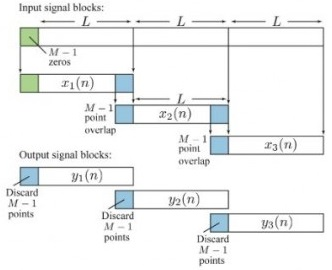
\includegraphics[width=.7\textwidth]{Immagini/ols}
	\caption{Metodo Overlap and Save}
	\label{fig:ols}
\end{figure}

\section{Codice Matlab}

\section{Codice C}

\clearpage

\nocite{*}
%Il comando \printbibliography produce la sezione bibliografica con relativi
%titolo e testatina. Per mandarne il relativo titolo nell’indice generale si
%usa l’istruzione:
\printbibliography

\end{document} 